\documentclass[article]{jss}
\usepackage[utf8]{inputenc}

\providecommand{\tightlist}{%
  \setlength{\itemsep}{0pt}\setlength{\parskip}{0pt}}

\author{
Ítalo Ramos Cegatta\\University of São Paulo \And Cristian Villegas\\University of São Paulo
}
\title{comp3: um pacote em \proglang{R} para índices de competição em árvores
indivuais}
\Keywords{floresta, índice de competição, árvore individual, \proglang{R}}

\Abstract{
The abstract of the article.
}

\Plainauthor{Ítalo Ramos Cegatta, Cristian Villegas}
\Plaintitle{comp3}
\Shorttitle{comp3: um pacote em \proglang{R} para índices de competição em árvores
indivuais}
\Plainkeywords{floresta, índice de competição, árvore individual, R}

%% publication information
%% \Volume{50}
%% \Issue{9}
%% \Month{June}
%% \Year{2012}
\Submitdate{}
%% \Acceptdate{2012-06-04}

\Address{
    Ítalo Ramos Cegatta\\
  University of São Paulo\\
  First line Second line\\
  E-mail: \href{mailto:italocegatta@gmail.com}{\nolinkurl{italocegatta@gmail.com}}\\
  URL: \url{http://italocegatta.github.io}\\~\\
    }

\usepackage{amsmath}

\begin{document}

\section{Introdução}\label{introducao}

A construção de modelos de crescimento é essencial para o planejamento
florestal. Independente da abordagem do modelo, seja ele baseado em
processo, empírico ou híbrido, o objetivo é representar o crescimento de
árvores e povoamentos através de formulações matemáticas (BURKHART;
TOMÉ, 2012).

O crescimento de árvores individuais é influenciado por fatores como
idade, tamanho, microambiente, características genéticas e competição
(TOMÉ, 1988). Os modelos que representam este crescimento podem ser
construídos em função da idade, índice de sítio e o status competitivo,
sendo este último o mais difícil de ser definido e mensurado
quantitativamente (ZHANG; BURKHART; AMATEIS, 1996).

A competição pode ser definida pela interação entre indivíduos que
competem por recursos e por esse motivo há redução de sobrevivência,
crescimento e reprodução (BEGON; TOWNSEND; HARPER, 2006).

Entende-se que existem 3 motivos pelos quais se justificam o estudo da
competição no componente arbóreo de uma floresta: (i) como suporte às
decisões de manejo, onde informações facilmente coletadas em campo
indicam o potencial de crescimento após uma interferência silvicultural;
(ii) para entender qual a ordem e grandeza de influência de fatores como
água, luz, densidade populacional e nutrientes no crescimento de uma
árvore no povoamento; (iii) para a utilização de índices de competição
em modelos de predição com estimativa acurada do incremento em diâmetro
e altura das árvores (MORAVIE; DURAND; HOULLIER, 1999).

Em um modelo de crescimento de árvore individual, o índice de competição
caracteriza o grau em que o espaço disponível para crescimento de uma
planta é compartilhado pelas suas vizinhas (BURTON, 1993; RADTKE;
WESTFALL; BURKHART, 2003). A avaliação da performance dos índices de
competição é comumente realizada através da correlação do índice com o
incremento em diâmetro, área basal e altura (DANIELS; BURKHART; CLASON,
1986). Diversos autores, ao modelar o crescimento e a produção,
obtiveram ganhos na qualidade do ajuste ao incluir índices de competição
no modelo (MORAVIE; DURAND; HOULLIER, 1999; SCHRÖDER; GADOW, 1999;
SOARES; TOMÉ, 1999; CONTRERAS; AFFLECK; CHUNG, 2011; FRAVER et al.,
2014)

É comum na literatura a classificação dos índices de competição em dois
grupos: dependentes e independentes da distância (MALEKI; KIVISTE;
KORJUS, 2015). Índices independentes da distância não necessitam das
coordenadas das árvores, uma vez que são simples cálculos envolvendo
variáveis do povoamento e da árvore-objeto. Já os dependentes da
distância consideram as dimensões e localização parcial dos vizinhos
competidores para o cálculo do índice. Para este índice, também é
necessário um critério que define quais árvores são competidoras em
relação a uma data árvore-objeto. (SOARES; TOMÉ, 1999; RIVAS et al.,
2005).

\section{The comp3 package}\label{the-comp3-package}

O software R é um ambiente computacional para desenvolvimento de
análises estatísticas e gráficas (R CORE TEAM, 2016), a linguagem dispõe
de várias funções para análises de dados e ainda possibilita utilizar
funções disponíveis em pacotes criados por outros usuários. O CRAN,
principal repositório de pacotes da linguagem R possui poucos pacotes
direcionados para resolução de problemas da área florestal, com destaque
para os pacotes \emph{FAwR} e \emph{lmfor}. O pacote \emph{comp3} foi
desenvolvido com o objetivo de disponibilizar funções que facilitam o
cálculo de índices de competição de árvores individuais de um povoamento
florestal. Estão implementados os principais índices de competição tanto
para florestas plantadas quanto para florestas naturais. A concepção das
funções do pacote sugere um fluxo de trabalho para o calculo dos
índices, que envolve:

\begin{itemize}
\item
  criação de coordenadas locais para árvores que estejam dispostas em
  parcelas rigorosamente esquadrejada;
\item
  delimitação da faixa de bordadura da parcela, que identifica as
  árvores como úteis para análise e as árvores de bordadura;
\item
  determinação das árvores competidoras para cada árvore-objeto;
\item
  cálculo de índices dependentes ou independentes da distância.
\end{itemize}

\subsection{Coordenadas locais}\label{coordenadas-locais}

Caso o banco de dados não possua a disposição espacial das árvore, mas
se sabe que as árvores da parcela amostral foram plantadas com extremo
rigor e esquadrejamento, é possível criar um grid hipotético e assim
gerar coordenadas locais para as árvores da parcela.

O exemplo abaixo exemplifica a criação de coordenadas para um conjunto
de dados hipotéticos. Pretende-se criar as coordenadas x e y de 25
árvores que pertencem a uma parcela de 5 linhas por 5 plantas. A
identificação de cada árvore é data pelo caminhamento em zig-zag pela
parcela. As funções \emph{xcoord} e \emph{ycoord} criam as coordenadas
locais a partir do identificador da árvore, podendo ele ser numérico ou
textual. É preciso especificar o arranjo de plantio e o número de linhas
que a parcela possui. Por fim, é definido o início do caminhamento,
podendo ser escolhido um dos quatro vértices da parcela.

\begin{CodeChunk}
\begin{CodeInput}
library(tidyverse)
library(comp3)

foo <- data_frame(id = paste0("arv.", 1:25)) %>% 
  mutate(
    x = xcoord(x = id, xspacing =  2, ncol =  5, star = "left-bottom"),
    y = ycoord(x = id, yspacing =  2, ncol =  5, star = "left-bottom")
  )

ggplot(foo, aes(x, y, label = id)) +
  geom_text(show.legend = FALSE)
\end{CodeInput}


\begin{center}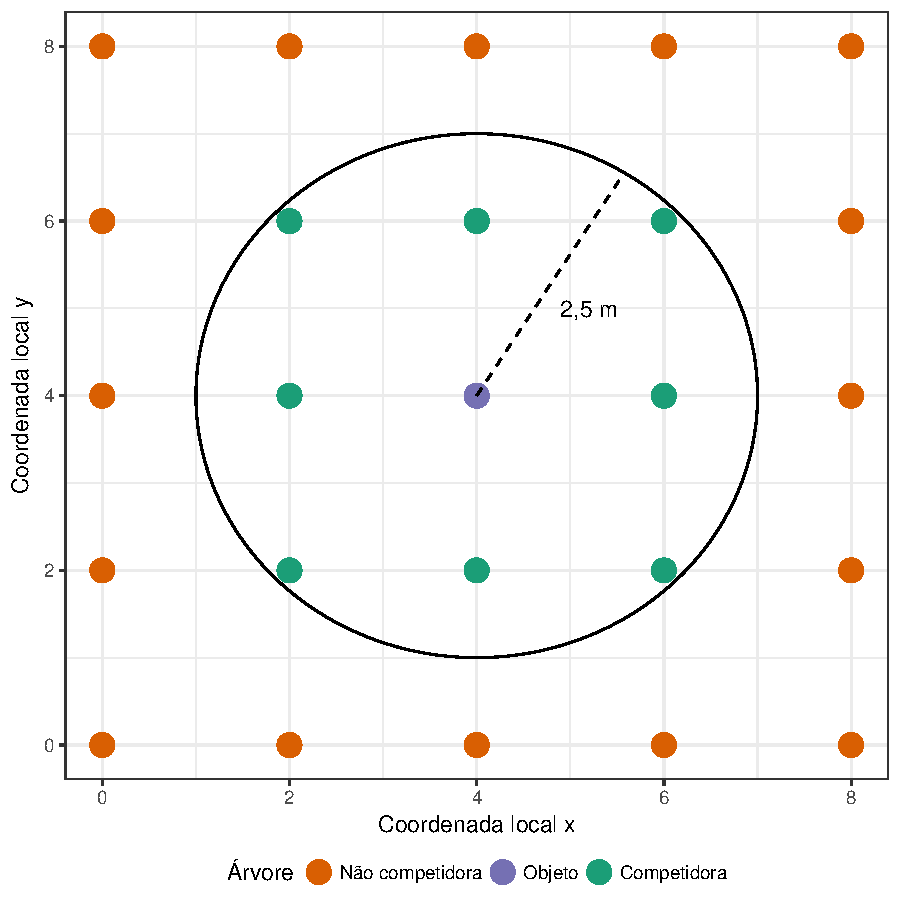
\includegraphics{comp3-paper_files/figure-latex/unnamed-chunk-1-1} \end{center}

\end{CodeChunk}

\subsection{Índices de competição}\label{indices-de-competicao}

Foram implementados índices dependentes e independentes da distância.
Cada índice, identificado com o nome do autor que o propôs, tem uma
função própria e é calculado individualmente. Os índices independentes
da distância necessitam obrigatoriamente do diâmetro das árvores e
eventualmente da área da parcela amostral. Já os índices dependentes da
distância exigem além do diâmetro, as coordenadas das árvores em um
plano cartesiano, seja ele real ou hipotético, e do método que considera
uma árvore vizinha como competidora.

\subsection{selection of competitors}\label{selection-of-competitors}

Para determinar se uma árvore é competidora em relação à árvore-objeto,
é necessário determinar ou o raio de busca que tem como centro a
árvore-objeto, ou especificar as n árvores mais próximas que serão
consideradas como competidoras. A Figura 1 mostra 25 árvores
hipotéticas, dispostas de maneira regular. A partir da árvore objeto,
todas as árvores vizinhas que estiverem dentro do circulo com raio de
2,5 m são consideradas como competidoras. A determinação do raio de
busca ou do número de arvores mais próximas é determinada pelo
pesquisador e tem impacto relevante no cálculo dos índices dependentes
da distância.

\section{Case study}\label{case-study}



\end{document}

